\chapter{Progettazione}

\section{Concettualizzazione}
Dopo aver raccolto ed analizzato i requisiti, è necessario individuare gli oggetti del dominio e quali sono le loro proprietà e le relazioni tra di essi, codificandoli opportunamente in un formalismo logico.

%I concetti che risaltano fanno riferimento al glossario in \ref{sec:glossary}. Vengono riportati con la loro rappresentazione logica:

\begin{figure}[htb]
	\centering
	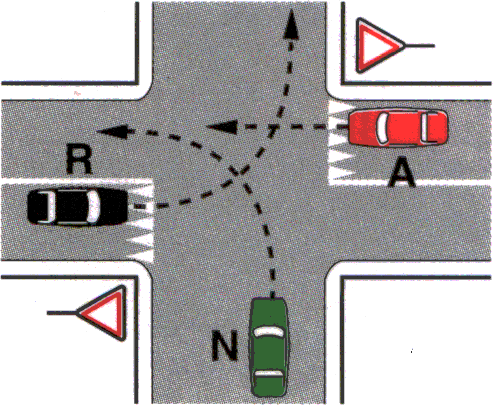
\includegraphics[width=.5\textwidth]{images/example}
	\caption{Esempio di incrocio}
\end{figure}


Osservando l'immagine, si può procedere all'estrazione delle informazioni necessarie per costruire il sistema.

\subsection{Universo}

I veicoli sono caratterizzati dal loro colore, o dalla loro tipologia o una qualsiasi informazione utile per differenziarli. Inoltre si vuole conoscere da dove vengono e dove sono diretti, in particolare se hanno svoltato o hanno proseguito dritto. Occorre rappresentare anche la direzione e i bracci dell'incrocio.

Per identificare questo tipo di informazioni, una costruzione sensata potrebbe essere:
\begin{verbatim}
proviene(veicolo(nero), braccio(ovest)).
transita(veicolo(nero), sinistra, braccio(nord)).
\end{verbatim}

La struttura \texttt{proviene} ci indica quale veicolo va in un determinato braccio. Il predicato \texttt{veicolo} ha come operando un atomo che descrive in modo chiaro una caratteristica della macchina. Si potrebbe anche usare la lettera che accompagna l'auto nell'immagine, così da ottenere \texttt{veicolo(r)} (non maiuscola, altrimenti verrebbe scambiata per una variabile). Il braccio sfrutta le \textbf{direzioni} della rosa dei venti, in questo caso \texttt{ovest}. Le direzioni possibili sono otto, come in figura:

\begin{figure}[htb]
	\centering
	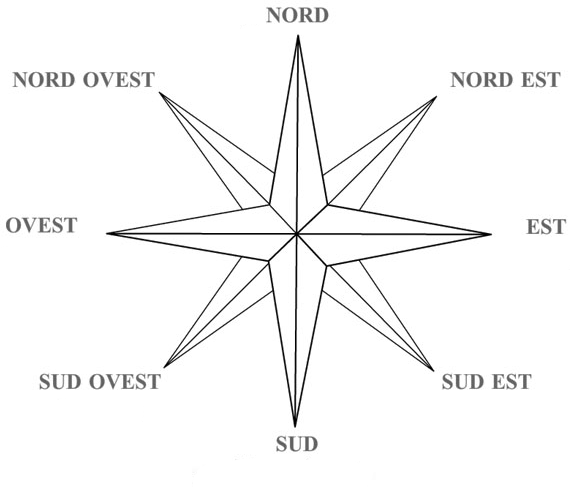
\includegraphics[width=.5\textwidth]{images/rose}
	\caption{Rosa dei venti}
\end{figure}

